\documentclass[10pt, aspectratio=169]{beamer}
\usetheme{Madrid}
\usecolortheme{whale}

% --- Paquetes Fundamentales ---
\usepackage[utf8]{inputenc}
\usepackage[spanish]{babel}
\usepackage{booktabs}
\usepackage{amsmath}
\usepackage{tikz}
\usepackage{subfig}
\usetikzlibrary{trees, positioning, arrows.meta}
\usepackage{booktabs}

% --- Configuración de Colores Personalizados (Estilo Banca Corporativa) ---
\definecolor{DeepBlue}{RGB}{0, 45, 114}
\definecolor{MidBlue}{RGB}{0, 80, 136}
\setbeamercolor{structure}{fg=DeepBlue}
\setbeamercolor{title}{fg=white, bg=DeepBlue}

\author[]{\texorpdfstring{César Núñez Cuevas\newline\url{cnunezc@fen.uchile.cl}}{Author}}
\title{\textbf{Ciencia de Datos para las Finanzas}}
%\setbeamercovered{transparent} 
%\logo{} 
%\institute{Facultad de Economía y Negocios\\Universidad de Chile} 
\date{} 
\subtitle{Introducción a la Ciencia de datos para las Finanzas}
\setbeamertemplate{navigation symbols}{} 
\titlegraphic{
\includegraphics[width=3.0cm]{images.png}}

\begin{document}
	
	%%%Portada%%%
	\begin{frame}
		\titlepage
	\end{frame}
	%%%%%%%%%%%%%
	
	%%%%%%%%%%%%%%%%%%%%%%%%%%%%%%%%%%%%%%%%%%
	
	%%%%%%%%%%%%%%%%%%%%%%%%%%%%%%%%%%%%%%%%%%
	
	% ==============================================================================
	\section{I. El Funnel de Originación de Créditos}
	% ==============================================================================
	% Slide 3: Introducción a la Originación
	\begin{frame}{¿A quién no le ha pasado esto?}
		\centering
		
\includegraphics[width=12.0cm]{1.png}
	\end{frame}
	
	% Slide 3: Introducción a la Originación
	\begin{frame}{¿Qué es el Proceso de Originación?}
		\begin{block}{Definición Operacional}
			La \textbf{originación de crédito} es el conjunto de etapas por las cuales pasa un cliente desde que manifiesta interés en un producto de financiamiento hasta que los fondos son desembolsados.
		\end{block}
		\vspace{0.3cm}
		\begin{itemize}
			\item Requiere un equilibrio crítico entre la \textbf{experiencia de usuario (UX)} (rapidez) y la \textbf{gestión del riesgo} (precisión).
			\item Históricamente basado en comités y reglas manuales; hoy automatizado a través de modelos analíticos.
		\end{itemize}
	\end{frame}
	
	% Slide 4: Anatomía del Funnel de Crédito
	\begin{frame}{Las Etapas de la Cascada de Crédito}
		\centering
		
\includegraphics[width=13.0cm]{2.png}
	\end{frame}
	
	% Slide 6: Concepto de Oferta Pre-aprobada
	\begin{frame}{La Oferta Pre-aprobada}
		\begin{itemize}
			\item \textbf{Inversión del flujo:} En lugar de esperar a que el cliente pida un monto, el banco calcula de forma proactiva su capacidad antes del contacto.
			\item Genera estrategias de \textit{cross-selling} efectivas en aplicaciones web y móviles.
			\item El éxito depende de un motor predictivo que asigne el \textbf{monto óptimo} sin disparar la tasa de default.
		\end{itemize}
	\end{frame}
	
	% ==============================================================================
	\section{II. Modelos de Aprendizaje Supervisado}
	% ==============================================================================
	% Slide 7: ¿Qué es el Aprendizaje Supervisado?
	\begin{frame}{¿Cómo entra el Machine Learning acá?}
		\centering
		\includegraphics[width=.10]{Darth-Vader-introduction-in-Star-Wars-A-New-Hope.png}
	\end{frame}
	
	
	% Slide 7: ¿Qué es el Aprendizaje Supervisado?
	\begin{frame}{Fundamentos del Aprendizaje Supervisado}
		\begin{block}{Concepto Core}
			Algoritmos que aprenden a partir de un conjunto de datos históricos que contiene tanto las características del cliente (\textbf{Features}) como el resultado real observado en el pasado (\textbf{Target} o Etiqueta).
		\end{block}
		\vspace{0.4cm}
		\begin{equation*}
			Y = f(X) + \epsilon
		\end{equation*}
		Donde $X$ representa el vector de características del solicitante e $Y$ representa si pagó o entró en mora.
	\end{frame}
	
	% Slide 8: Componentes: Características y Etiquetas
	\begin{frame}{Componentes del Dataset en Crédito}
		\begin{columns}
			\begin{column}{0.5\textwidth}
				\begin{exampleblock}{Variables Predictoras ($X$ - Features)}
					\begin{itemize}
						\item Historial de comportamiento de pagos.
						\item Nivel de ingresos declarados.
						\item Nivel de endeudamiento consolidado.
						\item Estabilidad y antigüedad laboral.
					\end{itemize}
				\end{exampleblock}
			\end{column}
			\begin{column}{0.5\textwidth}
				\begin{alertblock}{Variable Objetivo ($Y$ - Target)}
					\begin{itemize}
						\item Variable Binaria ($0$ o $1$).
						\item $1$ = Crédito Aprobado / Buen Pagador.
						\item $0$ = Crédito Rechazado / Cliente con Default.
					\end{itemize}
				\end{alertblock}
			\end{column}
		\end{columns}
	\end{frame}
	
	% Slide 9: Clasificación vs. Regresión en Originación
	\begin{frame}{Tipos de Problemas en el Modelado de Crédito}
		En nuestro flujo de originación conviven ambos enfoques:
		\vspace{0.3cm}
		\begin{enumerate}
			\item \textbf{Clasificación (Salida Cualitativa):} Determinar si el cliente califica o no para la oferta (\textbf{SÍ/NO}).
			\item \textbf{Regresión (Salida Cuantitativa):} Si el cliente es aprobado, determinar matemáticamente cuánta línea de crédito otorgar (\textbf{Monto asignado en \$}).
		\end{enumerate}
	\end{frame}
	
	% Slide 10: La importancia del Train/Test Split
	\begin{frame}{La Estrategia del Data Split (70/30)}
		Para medir la capacidad real del modelo, dividimos de forma estricta los datos históricos:
		\vspace{0.4cm}
		\begin{itemize}
			\item \textbf{70\% - Datos de Entrenamiento (Train):} Utilizados por el algoritmo para encontrar las reglas de segmentación y construir el árbol.
			\item \textbf{30\% - Datos de Validación/Test:} Datos retenidos que el modelo jamás ha visto. Sirven para comprobar si el árbol generaliza correctamente o si sufrió de \textit{overfitting} (memorización).
		\end{itemize}
	\end{frame}
	
	% Slide 11: ¿Qué es el Overfitting en Riesgo de Crédito?
	\begin{frame}{El Peligro del Sobreajuste (Overfitting)}
		\begin{itemize}
			\item Ocurre cuando un árbol crece demasiado y crea reglas tan específicas que solo funcionan para el set de entrenamiento.
			\item \textbf{Consecuencia financiera:} El modelo se vuelve incapaz de clasificar nuevos clientes del mercado real, subestimando el riesgo y provocando pérdidas por impagos.
		\end{itemize}
	\end{frame}
	
	% ==============================================================================
	\section{III. Definición de los Datos y Variables}
	% ==============================================================================
	
	% Slide 12: Las 5 Variables Clave del Ejercicio
	\begin{frame}{Definición de las Variables en el Dataset}
		Para construir nuestro modelo en Python y Excel, analizamos 5 variables fundamentales:
		\vspace{0.3cm}
		\begin{table}[]
			\small
			\begin{tabular}{lll}
				\toprule
				\textbf{Variable} & \textbf{Tipo} & \textbf{Descripción} \\ \midrule
				Historial\_Crediticio & Categórica & Comportamiento de pago previo (Bueno, Regular, Malo) \\
				Nivel\_Ingresos & Categórica & Rango salarial bruto mensual (Altos, Medios, Bajos) \\
				Relacion\_Deuda\_Ingreso & Numérica & Porcentaje del salario destinado a pagar deudas actuales \\
				Antiguedad\_Laboral & Numérica & Años de permanencia en el trabajo actual \\
				Monto\_Solicitado & Numérica & Línea de financiamiento requerida por el cliente \\ \bottomrule
			\end{tabular}
		\end{table}
	\end{frame}
	
	% Slide 13: Variable 1 y 2: Historial e Ingresos
	\begin{frame}{Variable Core: Historial Crediticio e Ingresos}
		\begin{itemize}
			\item \textbf{Historial Crediticio:} Es estadísticamente el predictor de riesgo más fuerte (medido por el indicador Gini en la industria). Refleja el \textit{willingness to pay} (voluntad de pago).
			\item \textbf{Nivel de Ingresos:} Representa el \textit{ability to pay} (capacidad financiera bruta). Define el tamaño potencial de la oferta.
		\end{itemize}
	\end{frame}
	
	% Slide 14: Variable 3: Relación Deuda/Ingreso (DTI)
	\begin{frame}{Carga Financiera: Relación Deuda/Ingreso (DTI)}
		\begin{block}{Fórmula Clave de Riesgo}
			\begin{equation*}
				\text{DTI} = \frac{\text{Total de Deudas Mensuales Consolidadas}}{\text{Ingreso Bruto Mensual}}
			\end{equation*}
		\end{block}
		\begin{itemize}
			\item Un DTI superior al $65\%$ indica que el cliente está financieramente sobrecargado, operando habitualmente como un criterio de rechazo directo.
		\end{itemize}
	\end{frame}
	
	% Slide 15: Variable 4 y 5: Estabilidad y Magnitud
	\begin{frame}{Antigüedad Laboral y Monto Solicitado}
		\begin{itemize}
			\item \textbf{Antigüedad Laboral:} Funciona como mitigador del riesgo de desempleo repentino. Estabilidad en el empleo reduce la variabilidad del ingreso.
			\item \textbf{Monto Solicitado:} Es la ancla comercial del modelo. El árbol debe evaluar si el monto solicitado guarda proporción lógica con el perfil de ingresos del cliente.
		\end{itemize}
	\end{frame}
	
	% Slide 16: Formulación de la Salida Comercial
	\begin{frame}{Definición de las Variables de Destino}
		El modelo entregará dos salidas estructuradas en cascada:
		\vspace{0.3cm}
		\begin{itemize}
			\item \textbf{Salida 1: Oferta\_Aprobada (SÍ/NO):} Clasificación binaria pura basada en la calidad del riesgo del cliente.
			\item \textbf{Salida 2: Monto\_Preaprobado (\$):} Asignación analítica de la línea de crédito ajustada por capacidad y riesgo (Monto máximo vs. cupo básico).
		\end{itemize}
	\end{frame}
	
	% ==============================================================================
	\section{IV. El Árbol de Decisión Ilustrado}
	% ==============================================================================
	
	% Slide 17: ¿Cómo funciona un Árbol de Decisión?
	\begin{frame}{La Lógica Secuencial de los Árboles}
		\begin{itemize}
			\item Funciona mediante reglas de partición binaria recursiva.
			\item Comienza en un \textbf{Nodo Raíz} que selecciona la variable que aporta la mayor separación de riesgo.
			\item Se ramifica hacia \textbf{Nodos Internos} y culmina en \textbf{Nodos Hoja}, que dictan la predicción definitiva del perfil.
		\end{itemize}
	\end{frame}
	
	% Slide 18: El Árbol de Decisión Ilustrado (Corregido y Optimizado)
	\begin{frame}{El Árbol de Decisión del Flujo de Crédito}
		\centering
		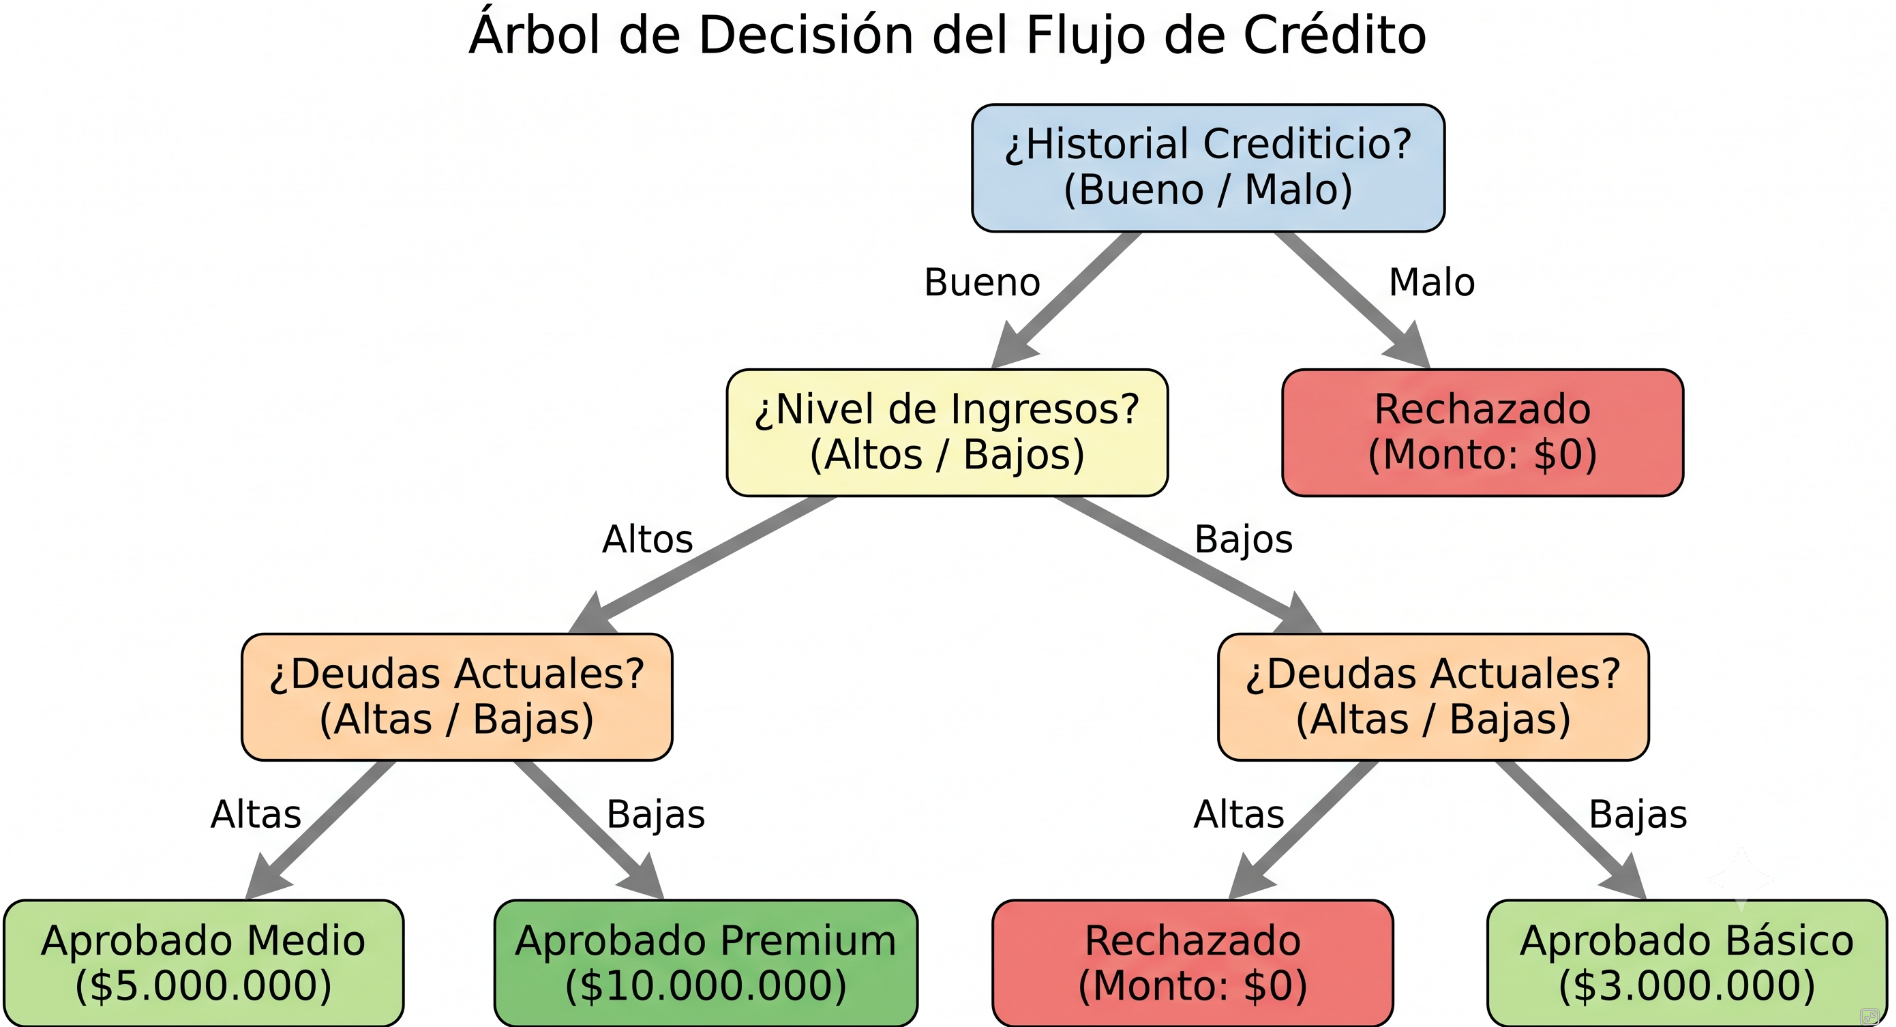
\includegraphics[width=12.0cm]{Gemini_Generated_Image_vrtv3nvrtv3nvrtv.png}
	\end{frame}
	
	% Slide 19: Criterio de Selección de Splits
	\begin{frame}{¿Cómo decide el modelo dónde cortar la muestra?}
		El modelo utiliza criterios estadísticos de pureza matemática para elegir la variable óptima en cada paso:
		\vspace{0.3cm}
		\begin{itemize}
			\item \textbf{Impureza de Gini:} Mide la probabilidad de clasificar incorrectamente un registro del set de datos. El algoritmo busca minimizar esta métrica en cada rama.
			\item \textbf{Entropía (Ganancia de Información):} Mide el desorden o la aleatoriedad de los datos. Buscamos nodos hijos lo más homogéneos (puros) posibles.
		\end{itemize}
	\end{frame}
	
	% Slide 20: Ventajas de la Arquitectura de Árbol
	\begin{frame}{¿Por qué los Bancos usan Árboles de Decisión?}
		\begin{itemize}
			\item \textbf{Explicabilidad Total (White Box):} A diferencia de las redes neuronales, es fácil explicar a un regulador o auditor el camino exacto que causó la denegación de un crédito.
			\item \textbf{Manejo de No-Linealidad:} Captura de forma nativa interacciones complejas entre variables categóricas y numéricas sin requerir transformaciones matemáticas avanzadas.
		\end{itemize}
	\end{frame}
	
	% Slide 21: Limitaciones Teóricas
	\begin{frame}{Limitaciones del Árbol Individual}
		\begin{itemize}
			\item \textbf{Inestabilidad (Alta Varianza):} Pequeños cambios en los datos de entrenamiento pueden dar lugar a un árbol completamente diferente.
			\item Es por esto que en la producción avanzada de la industria se migra hacia ensamblados como \textit{Random Forests} o \textit{XGBoost}.
		\end{itemize}
	\end{frame}
	
	% ==============================================================================
	\section{V. Salida de Resultados y Lógica de Negocio}
	% ==============================================================================
	
	% Slide 22: Mapeo de la Matriz de Decisiones
	\begin{frame}{Matriz Logicial de Resultados}
		\begin{table}[]
			\small
			\begin{tabular}{ccccc}
				\toprule
				\textbf{Historial} & \textbf{Ingresos} & \textbf{Deudas} & \textbf{Oferta Aprobada} & \textbf{Monto Pre-aprobado} \\ \midrule
				Bueno & Altos & Bajas & \textbf{SÍ} & \$10.000.000 (Premium) \\
				Bueno & Altos & Altas & \textbf{SÍ} & \$5.000.000 (Medio) \\
				Bueno & Bajos & Bajas & \textbf{SÍ} & \$3.000.000 (Básico) \\
				Bueno & Bajos & Altas & \textbf{NO} & \$0 (Rechazo por Carga) \\
				Malo & Cualquiera & Cualquiera & \textbf{NO} & \$0 (Rechazo Político) \\ \bottomrule
			\end{tabular}
		\end{table}
	\end{frame}
	
	% Slide 23: Definición del Algoritmo del Monto
	\begin{frame}{Determinación Analítica del Monto}
		El monto asignado no es aleatorio, responde a una función estructurada:
		\vspace{0.3cm}
		\begin{block}{Lógica Algorítmica}
			$\text{Monto} = f(\text{Riesgo Base}) \times \text{Capacidad de Pago Disponible}$
		\end{block}
		\vspace{0.2cm}
		Mitiga el riesgo de \textit{Default} cortando la exposición del banco ante la combinación de variables desfavorables.
	\end{frame}
	
	% Slide 24: Implementación del Motor en Excel
	\begin{frame}[fragile]{Traducción del Árbol a Fórmulas de Excel}
		Para estudiantes sin experiencia en código, las ramas se transforman directamente en funciones lógicas anidadas:
		\vspace{0.4cm}
		\begin{exampleblock}{Fórmula para Oferta (Celda B10)}
			\texttt{=SI(B5="Malo"; "NO"; SI(Y(B5="Bueno"; B6="Bajos"; B7="Altas"); "NO"; "SÍ"))}
		\end{exampleblock}
		\vspace{0.3cm}
		\begin{exampleblock}{Fórmula para Monto (Celda B11)}
			\texttt{=SI(B10="NO"; 0; SI(Y(B6="Altos"; B7="Bajas"); 10000000; SI(Y(B6="Altos"; B7="Altas"); 5000000; 3000000)))}
		\end{exampleblock}
	\end{frame}
	
	% Slide 25: Conclusiones
	\begin{frame}{Conclusiones y Siguientes Pasos}
		\begin{itemize}
			\item Los árboles de decisión estructuran de forma gráfica y lógica las políticas comerciales de un banco.
			\item Pasar del diseño analítico en Excel al código en Python nos permite escalar estas reglas desde una matriz simple de 8 escenarios hasta millones de filas y múltiples combinaciones continuas.
		\end{itemize}
		\vspace{0.5cm}
		\centering
		\textbf{¡Muchas gracias! ¿Preguntas?}
	\end{frame}
	
\end{document}